\section {US Data Facility Architecture} \label{sec:usdfarch}


\begin{figure}
\begin{centering}
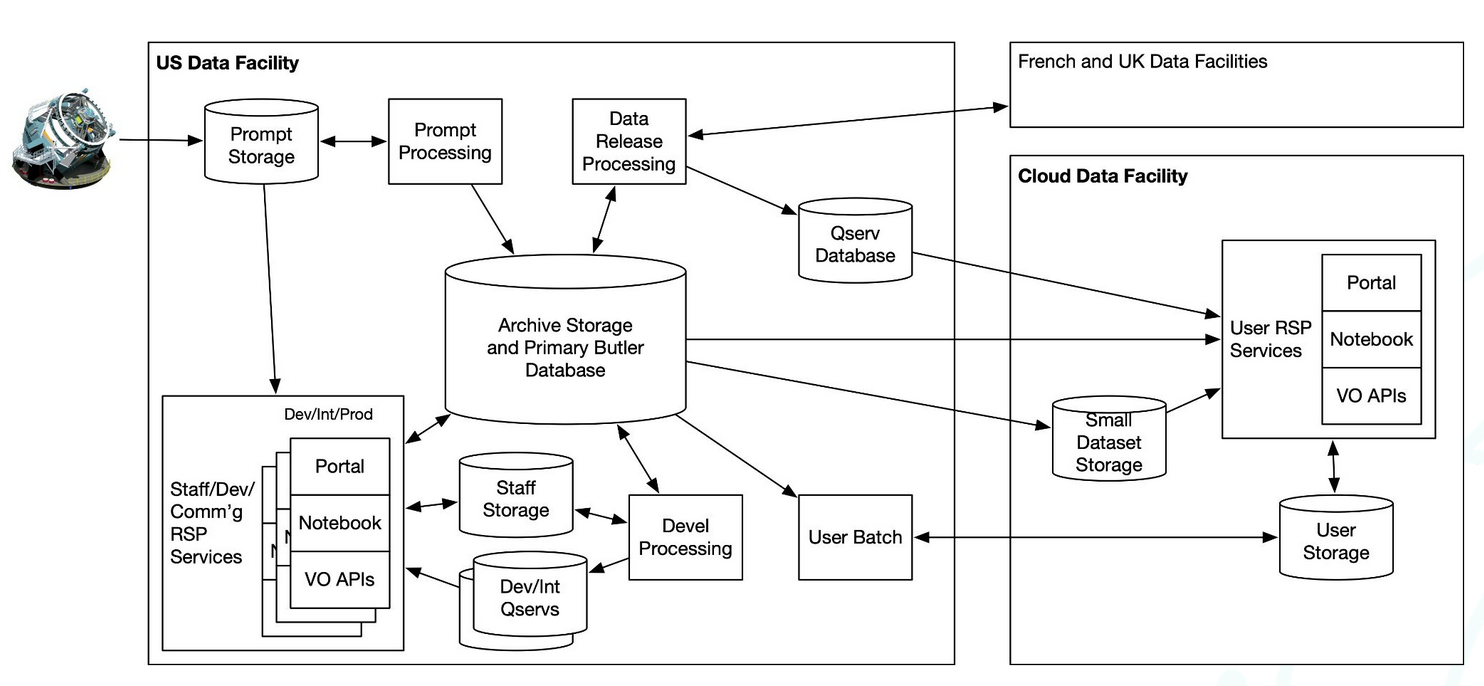
\includegraphics[width=0.9\textwidth]{hybrid}
	\caption{ Hybrid model: Data at SLAC but users on the cloud.  \label{fig:usdfarch}}
\end{centering}
\end{figure}

The scope for the USDF on-prem includes data production services:
prompt processing, serving alerts to the community and annual Data
Release Processing. The USDF acts as the archive for all data, and
provides the Qserv object catalog as well as access to image data, be
it cutouts or full images. It will provide batch cycles for cloud-based science users.
It will also act as a home for developers and staff (and
commissioners) to ensure data quality (see \autoref{fig:usdfarch}).


\subsection{Hardware}

The USDF is hosted by the SLAC Shared Scientific Data Facility
(S3DF) which is itself hosted in Stanford Research Computing Facility (SRCF).
SRCF accommodates projects from SLAC and Stanford, while the S3DF is the
focal system for SLAC projects. The USDF lives in a shared cluster and
benefits from economies of scale and standardization across S3DF
projects. It is also exposed to potentially disruptive activities by
other projects.

In order to support hundreds of PBs of storage, S3DF adopted the Weka
filesystem for high throughput. Weka is based on a tiered system with
Solid State Disks (SSD) backed by spinning disk. It presents a POSIX interface while the
backend is a Ceph object store. This system forms the basis of the
data archive. A tape robot provides storage for seldom-read data and
acts as a backup tier.

Batch processing is done on a Slurm cluster, currently primarily Advanced Micro Devices (AMD) milan
processors with 128 cores and 512 GB RAM per node.

Data is transported to the USDF from the summit over a combined
leased-line, ESNet-supported network with routing optimized via an
overlay. The leased line terminates in Atlanta, where ESNet takes
over. Traffic to the two other Data Facilities is also provided by
ESNet, connecting to the GEANT\footnote{pan-European data network for the research and education community}
 and Renater systems in Europe.

\subsection{Batch processing}

The USDF supports batch processing for a number of purposes: annual
multi-site data releases; pipelines teams testing for algorithms
performance; processing by individual developers for their algorithm
development; data quality checking and validation.

Multisite processing makes use of the Production ANd Distributed Analysis system (PanDA),\cite{2024CSBS....8....4M} developed
by ATLAS (A Toroidal LHC Apparatus) for the Large Hadron Colider (LHC).
It has a well-defined mechanism for routing work
from a central server to multiple remote locations. ATLAS has
demonstrated submitting millions of jobs per day to hundreds of sites.
A difference between typical astronomy and High Energy Physics (HEP) workflows is the
number of and duration of processes: astronomy tends to many more much
shorter jobs than HEP.\cite{2023arXiv231204921K} Significant effort was required working with the PanDA
team to cluster up short jobs to avoid prohibitive startup costs.
PanDA is a heavyweight solution to processing; local processing for
the pipelines teams and developers is done using HTCondor\footnote{\url{https://htcondor.org}}.

Data management and movement is also orchestrated by LHC tools: Rucio\footnote{\url{https://rucio.cern.ch}}
for data management and FTS3\footnote{\url{https://fts3-docs.web.cern.ch/fts3-docs/}} for movement. These tools also routinely
handle large numbers of files and transfers, however the difference between astronomy
and HEP persists here as well, with astronomy generating many more,
much smaller files than HEP. This will make the Rubin Rucio database
bigger than ATLAS's and will require some growth planning.

The large number of small files will also be a challenge for network
transfer. We are investigating zipping up large numbers of files both
for better transfer as well as easier storage on tape.

\subsection{Non-user-facing services}

Currently the primary reasons for putting services on-prem are a low
latency requirement for prompt processing, and the still-unfavorable
comparison of storage prices between on-prem and the cloud. To a lesser
degree, those comparisons also apply to CPU.

This means that Prompt Processing and Alerts production, with their
2-minute latency requirement are hosted on-prem. Additionally, there
are security requirements on data arriving at the USDF, including
physical measures implemented on the racks themselves.\cite{DMTN-199}

The large data volumes associated with the storage archive and Qserv
database hosted at the USDF implies that external access to them must be
provided by services.

Kubernetes is used to manage almost all our services, making use of
ArgoCD as well as our custom Phalanx system (see \S \ref{sec:deploy}).
Native Kubernetes tools
are used to manage standard services, such as Postgres databases,
making administration, backups, etc, scalable. Rucio and PanDA are
managed by Kubernetes to take advantage of these features.

The Prompt Processing framework executing the Alert Production is implemented
using Knative\footnote{\url{https://knative.dev/docs/}} on top of
Kubernetes to allow elastic instantiation, configuration, and teardown of
pods responding to notifications from the summit in advance of the
next visit.
Prompt Processing and Alert Distribution both use Kafka installed on Kubernetes.
We use the Strimzi Operator to install Kafka and for management.  Strimzi
has worked well to simplify installation, upgrades, and for maintaining
health of the Kafka clusters.

Three large database systems are minimally using Kubernetes, as they
are either commercial or custom services with no native Kubernetes
support. These are the Engineering and Facilities Database (EFD),\cite{2024SPIE13101.59Ftmp}
Qserv, and Cassandra systems, with Qserv the custom system.
The EFD is implemented with an InfluxDB Enterprise High Availability cluster.

For monitoring we use Prometheus\footnote{\url{https://prometheus.io}}.  Prometheus has native support for
Kubernetes metrics and many of the Kubernetes operators described earlier
like Strimzi and the Cloud Native Postgres (CNPG) natively provide metrics in Prometheus. We also
wrote some of our own metrics to track Prompt Processing.
We use Grafana for creating dashboards to visual metrics and for generating alarms when thresholds are crossed.
We use Loki from Grafana Labs to capture logs from Kubernetes pods
and from application level logs. Loki stores these logs in an on-premise S3 Ceph Cluster.
